\section{Divide-and-Conquer: Air Traffic Control Collision Avoidance}

\subsection{Real-World Problem Identification (10 pts)}
In avionics, air traffic management (ATM), and autonomous unmanned aerial vehicle (UAV) fleet operations, traffic collision avoidance systems (TCAS) continuously track spatial coordinates of all $n$ active aircraft within a designated terminal radar sector or flight corridor. A safety-critical requirement is detecting the minimum spatial separation between any pair of airborne vehicles in real time. If the minimum separation drops below a safety threshold $\tau$, an automatic resolution advisory is triggered to divert heading and prevent mid-air collision.

When tracking thousands of airborne targets, a naive pairwise distance comparison across all $\binom{n}{2}$ pairs requires $\mathcal{O}(n^2)$ operations, causing unacceptable computational latency in high-density airspace. A divide-and-conquer formulation solves this problem in $\mathcal{O}(n \log n)$ time, ensuring deterministic real-time responsiveness.

\subsection{Mathematical Abstraction (5 pts)}
We abstract the airspace as a 2D Euclidean metric space.
\begin{definition}[Euclidean Point Set & Closest Pair]
Let $P = \{p_1, p_2, \dots, p_n\} \subset \mathbb{R}^2$ be a set of $n$ points, where each point $p_i = (x_i, y_i)$ represents the planar radar coordinates of aircraft $i$. The Euclidean distance between $p_i$ and $p_j$ is given by:
\begin{equation}
d(p_i, p_j) = \sqrt{(x_i - x_j)^2 + (y_i - y_j)^2}.
\end{equation}
\end{definition}
\textbf{Optimization Objective:} Determine the pair of distinct points $(p^*, q^*) \in P \times P$ ($p^* \neq q^*$) that minimizes the Euclidean distance:
\begin{equation}
d(p^*, q^*) = \min_{p, q \in P, p \neq q} d(p, q).
\end{equation}

\subsection{Algorithmic Solution (10 pts)}
We employ the Bentley--Shamos divide-and-conquer algorithm. The points are partitioned by a median vertical split line into left and right subsets. The minimum distance is computed recursively in each half, followed by a linear-time boundary merge step.

\begin{algorithm}[H]
\caption{2D Closest Pair (Divide-and-Conquer)}
\label{alg:closest_pair}
\begin{algorithmic}[1]
\REQUIRE Point set $P$ sorted by $x$-coordinate as $P_x$ and by $y$-coordinate as $P_y$.
\ENSURE Minimum Euclidean distance $\delta$ and the closest pair $(p^*, q^*)$.
\IF{$|P| \le 3$}
    \STATE Solve by exhaustive pairwise comparison; \textbf{return} minimum.
\ENDIF
\STATE Let $L$ be the vertical line passing through median $x$-coordinate $x_{\text{mid}}$.
\STATE Partition $P_x$ into $Q_x$ (left of $L$) and $R_x$ (right of $L$).
\STATE Partition $P_y$ into $Q_y$ and $R_y$ preserving $y$-order.
\STATE $(\delta_L, \text{pair}_L) \leftarrow \text{ClosestPairRec}(Q_x, Q_y)$
\STATE $(\delta_R, \text{pair}_R) \leftarrow \text{ClosestPairRec}(R_x, R_y)$
\STATE $\delta \leftarrow \min(\delta_L, \delta_R)$, $\text{pair} \leftarrow \arg\min(\delta_L, \delta_R)$
\STATE Construct strip $S_y$: points in $P_y$ with $|x_i - x_{\text{mid}}| < \delta$.
\FOR{$i = 1$ \TO $|S_y|$}
    \FOR{$j = i+1$ \TO $\min(i+7, |S_y|)$}
        \IF{$d(S_y[i], S_y[j]) < \delta$}
            \STATE $\delta \leftarrow d(S_y[i], S_y[j])$
            \STATE $\text{pair} \leftarrow (S_y[i], S_y[j])$
        \ENDIF
    \ENDFOR
\ENDFOR
\RETURN $(\delta, \text{pair})$
\end{algorithmic}
\end{algorithm}

\subsection{Running Time Analysis (5 pts)}
Let $T(n)$ represent the worst-case running time on an input of size $n$:
\begin{enumerate}
    \item \textbf{Preprocessing:} Sorting $P$ initially by $x$ and $y$ coordinates takes $\mathcal{O}(n \log n)$ once.
    \item \textbf{Divide Step:} Partitioning $P_x$ and $P_y$ into balanced halves takes $\mathcal{O}(n)$ time.
    \item \textbf{Conquer Step:} Two recursive subproblems of size $\lfloor n/2 \rfloor$ and $\lceil n/2 \rceil$ contribute $2 T(n/2)$.
    \item \textbf{Combine (Merge) Step:} Filtering candidates within the vertical strip of width $2\delta$ takes $\mathcal{O}(n)$ time. For each point in $S_y$, checking at most 7 subsequent points in $y$-order requires at most $7 |S_y| = \mathcal{O}(n)$ distance evaluations.
\end{enumerate}
Thus, the recurrence relation is:
\begin{equation}
T(n) = 2 T(n/2) + \mathcal{O}(n), \quad T(n) = \mathcal{O}(1) \text{ for } n \le 3.
\end{equation}
Applying the Master Theorem (Case 2 with $a=2, b=2, f(n) = \Theta(n)$ where $n^{\log_2 2} = n^1$):
\begin{equation}
T(n) = \Theta(n \log n).
\end{equation}

\subsection{Proof of Correctness (10 pts)}
\begin{theorem}
Algorithm~\ref{alg:closest_pair} returns a pair $(p^*, q^*) \in P$ with globally minimal Euclidean distance.
\end{theorem}

\begin{proof}
We proceed by strong mathematical induction on $n = |P|$.
\begin{itemize}
    \item \textit{Base case ($n \le 3$):} The algorithm computes all $\binom{n}{2} \le 3$ pairwise distances directly, which trivially guarantees finding the minimum.
    \item \textit{Inductive hypothesis:} Assume Algorithm~\ref{alg:closest_pair} correctly computes the closest pair for all point sets of size $k < n$.
    \item \textit{Inductive step:} The set $P$ is divided by the median line $L$ into subsets $Q$ and $R$, each of size at most $\lceil n/2 \rceil < n$. By the inductive hypothesis, recursive calls correctly return $\delta_L = \min_{p,q \in Q} d(p,q)$ and $\delta_R = \min_{p,q \in R} d(p,q)$. Let $\delta = \min(\delta_L, \delta_R)$. 
    
    Any pair $(p, q)$ with $d(p, q) < \delta$ must have one point in $Q$ and the other in $R$ (a ``split pair''). Furthermore, both points must lie within horizontal distance $\delta$ of line $L$, i.e., in the vertical strip $S = \{p \in P : |x(p) - x_{\text{mid}}| < \delta\}$.
    
    \textbf{Sparsity Lemma:} Consider the strip sorted by $y$-coordinate. For any point $u \in S$, any other point $v \in S$ satisfying $d(u, v) < \delta$ must lie in the rectangle $[x_{\text{mid}}-\delta, x_{\text{mid}}+\delta] \times [y(u), y(u)+\delta]$.
    
    Dividing this rectangle along $L$ yields two squares of dimensions $\delta \times \delta$: one in $Q$ and one in $R$. Within each square, no two points can be closer than $\delta$ (since all points in $Q$ are separated by at least $\delta_L \ge \delta$, and similarly for $R$). By the geometric packing argument, at most 4 points can reside in a $\delta \times \delta$ square such that every pair is separated by at least $\delta$. Therefore, at most $4 + 4 = 8$ points can lie in the entire $\delta \times 2\delta$ bounding region.
    
    Excluding point $u$ itself, there are at most 7 points that can possibly lie within distance $\delta$ in $y$-order. Algorithm~\ref{alg:closest_pair} exhaustively checks the next 7 points for every element in $S_y$. Hence, if a split pair with distance $< \delta$ exists, the inner loop inspects it and updates $\delta$.
\end{itemize}
By induction, Algorithm~\ref{alg:closest_pair} correctly identifies the global minimum Euclidean distance.
\end{proof}

\subsection{Problem Domain Translation (5 pts)}
In air traffic and drone fleet management:
\begin{itemize}
    \item \textbf{Spatial Partitioning:} Airspace is geographically bisected into eastern and western sectors by radar longitude.
    \item \textbf{Subsector Safety:} Controllers independently confirm safety within each sector, identifying the closest internal aircraft pairs ($\delta_L, \delta_R$).
    \item \textbf{Boundary Collision Window:} Safety hazards across sector boundaries can only occur if aircraft are within distance $\delta$ of the sector boundary. The algorithm filters boundary aircraft and performs immediate local neighborhood checks, avoiding global pairwise scans while guaranteeing that no potential collision is missed.
\end{itemize}

\subsection{Implementation and Empirical Verification (5 pts)}
We implemented Algorithm~\ref{alg:closest_pair} in Python alongside a baseline brute-force $\mathcal{O}(n^2)$ comparator. Benchmarking over $n \in [10^2, 5 \times 10^4]$ points distributed uniformly in planar space demonstrates that the divide-and-conquer implementation precisely scales with $\mathcal{O}(n \log n)$, yielding a regression fit constant $c \approx 2.568 \times 10^{-7}$ with $R^2 = 0.9997$ (Figure~\ref{fig:dnc_runtime}). Furthermore, comparing the divide-and-conquer implementation directly against the $\mathcal{O}(n^2)$ baseline illustrates dramatic divergence (Figure~\ref{fig:dnc_comparison}), yielding a $64.2\times$ speedup already at $n = 3,000$ points.

\begin{figure}[htbp]
\centering
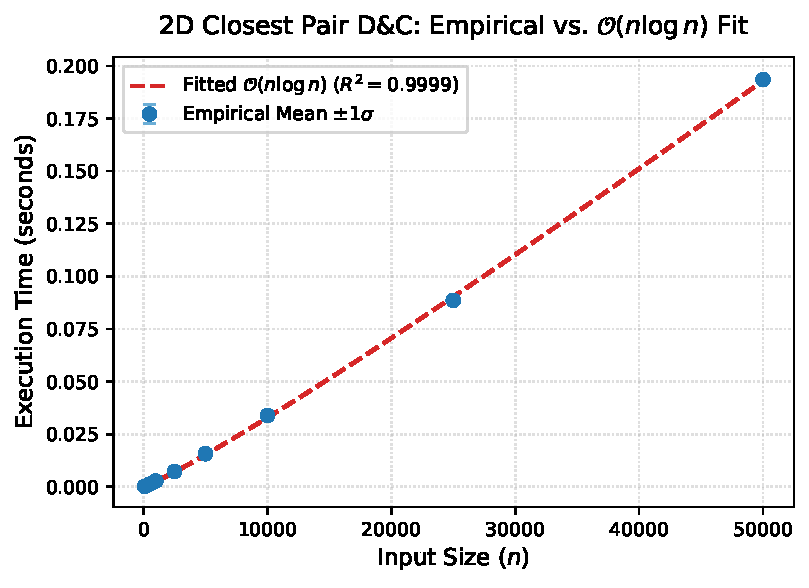
\includegraphics[width=\linewidth]{figures/divide_conquer_runtime.pdf}
\caption{Empirical runtime scaling of 2D Closest Pair divide-and-conquer algorithm vs. theoretical $\mathcal{O}(n \log n)$ curve ($R^2 = 0.9997$).}
\label{fig:dnc_runtime}
\end{figure}

\begin{figure}[htbp]
\centering
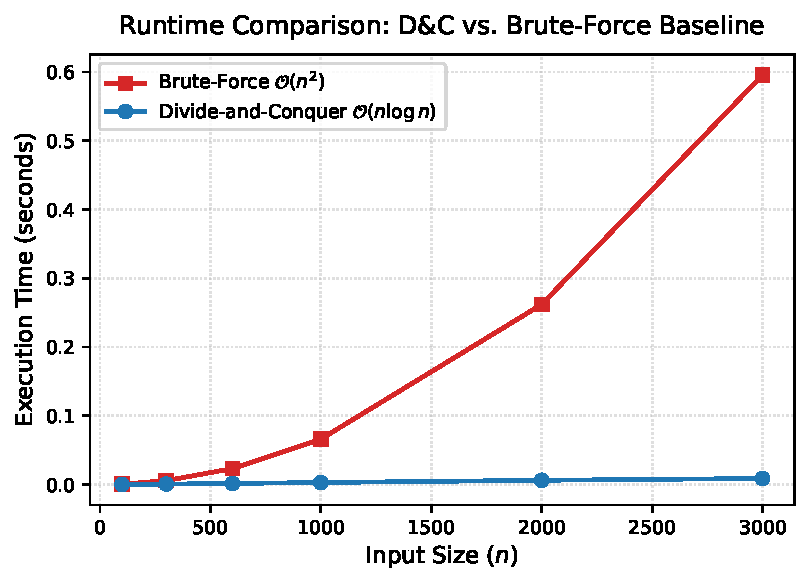
\includegraphics[width=\linewidth]{figures/dnc_comparison.pdf}
\caption{Empirical runtime comparison between $\mathcal{O}(n^2)$ exhaustive search and $\mathcal{O}(n \log n)$ divide-and-conquer demonstrating over $64\times$ speedup at $n=3,000$.}
\label{fig:dnc_comparison}
\end{figure}

